\subsection{Overview}

	As we anticipated, in this section we’re goint to give an array of views of our system, shaping it from many angles at once. We’ll detail both the high-level components and the interfaces interleaved among them, delving then into deployment and runtime view.
	[Check] The architectural style we chose to adopt is a three-layered one.
	The decision to implement an external DB was born because of the need of providing a realiable and safe synchronization tool for our users and to store other kinds of personal information submitted through the app (like preferences and the like).
	Since the client implements travel logic and actually consists in the mobile application we’re aiming to develop, we are without any doubt in the frame of a fat client design.
	
\subsection{Component View}
	The Component Diagram shown below describes the logical components of the system we are to develop, from a very high-level description on to a more detailed one. This diagram does not take into account the deployment phase, hence it doesn’t describe the logical layer of the system in terms of the physical tiers where it is deployed.

\begin{figure}[H]
		\centering
		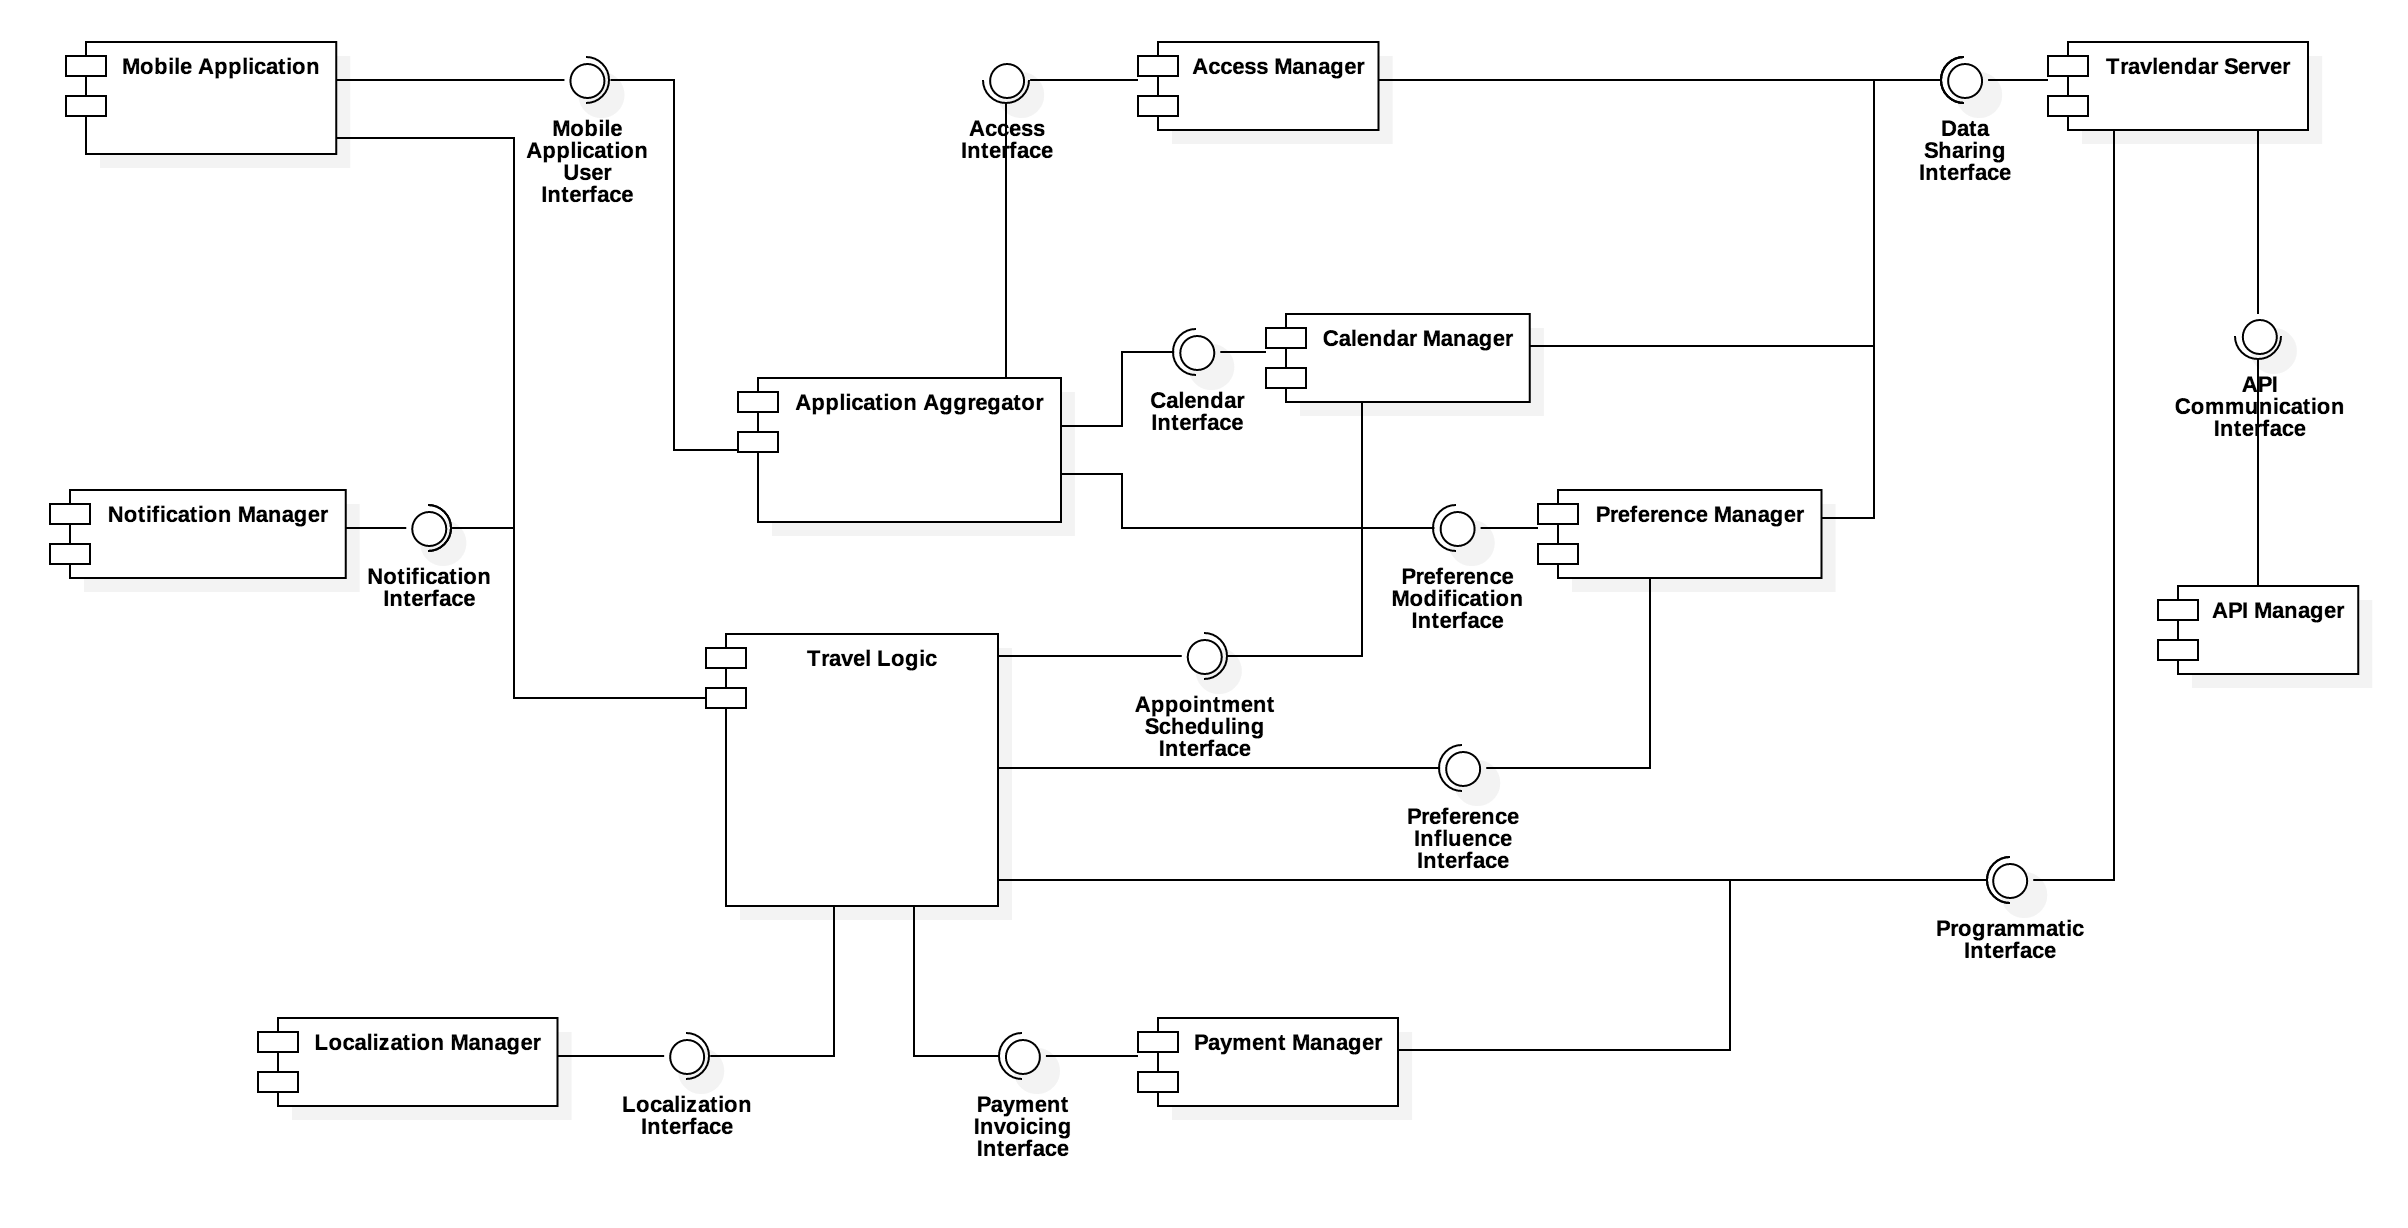
\includegraphics[width = \textwidth]{UML/componentDiagrams/highLevel}
		\caption{High level view}
		\label{componentHighLevel}
	\end{figure}

\paragraph{Mobile Application}
	This component represents the view of the User over its system. It’s split in two sub-components, Guest-view and User-view, which represents the two different ways an human interaction can be instaurated with the system.

	\begin{figure}[H]
		\centering
		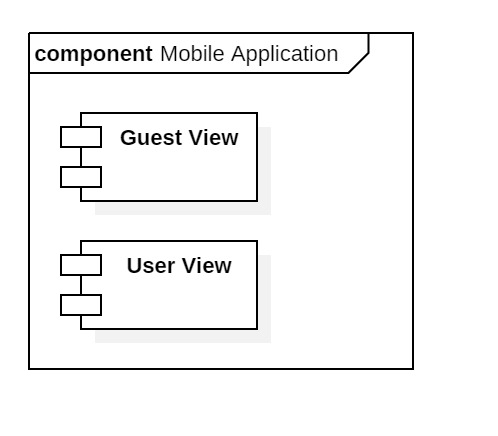
\includegraphics[scale = 0.2]{UML/componentDiagrams/mobileApplication}
	\end{figure}


\paragraph{Application Aggregator}
	This component works, unsuprisingly, as a collector of the different information \textit{Travlendar+} manages. It allows an easy management of every piece of information and allows us to avoid an high number of interfaces among the different components. 'Profile Manager' specifies the profile setting of the current user, while 'User Action Handler' allows us to register User's input.
	
	\begin{figure}[H]
		\centering
		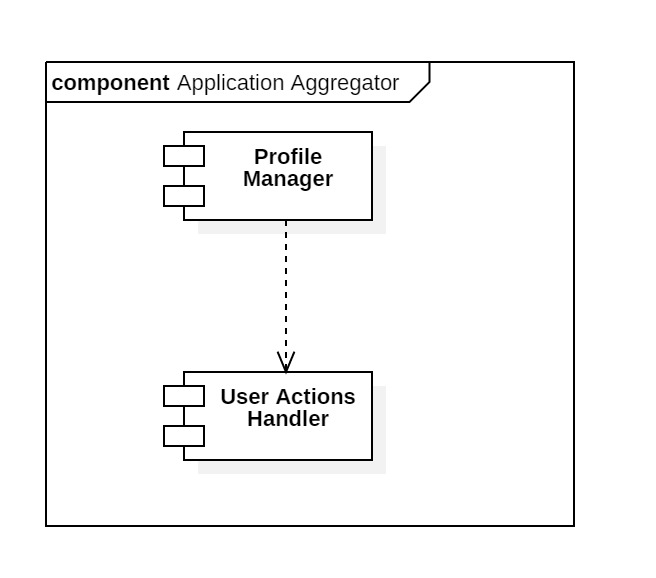
\includegraphics[scale = 0.2]{UML/componentDiagrams/applicationAggregator}
	\end{figure}
 
\paragraph{Calendar Manager}
	This component is divided into 'Appointments' and 'Breaks' sub-components, which track the appointments inserted by the User together with his breaks, and 'Trips', which is the list of trips arranged by the scheduler for every appointment. The sub-component 'Appointment Aggregator' serves the purpose of listing and presenting the content of the other two sub-components.
	
	\begin{figure}[H]
		\centering
		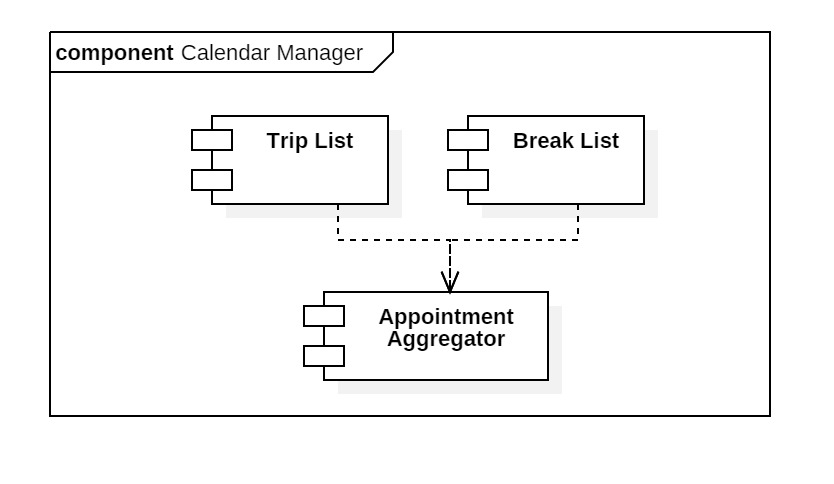
\includegraphics[scale = 0.2]{UML/componentDiagrams/calendarManager}
	\end{figure}
 

\paragraph{Preference Manager}
	This component serves the purpose of keeping track of the preferences expressed by the User. 'Season Pass Handler' takes care of storing season passes; 'Excluded Vehicles List' cuts off from the scheduler results involving a selection of banned transportation means, 'Preferences List' covers the remaining and wider spectrum of User's choices. 'Preference Handler' is the sub-component that manages the other ones and that communicates outside Preference Manager.

	\begin{figure}[H]
		\centering
		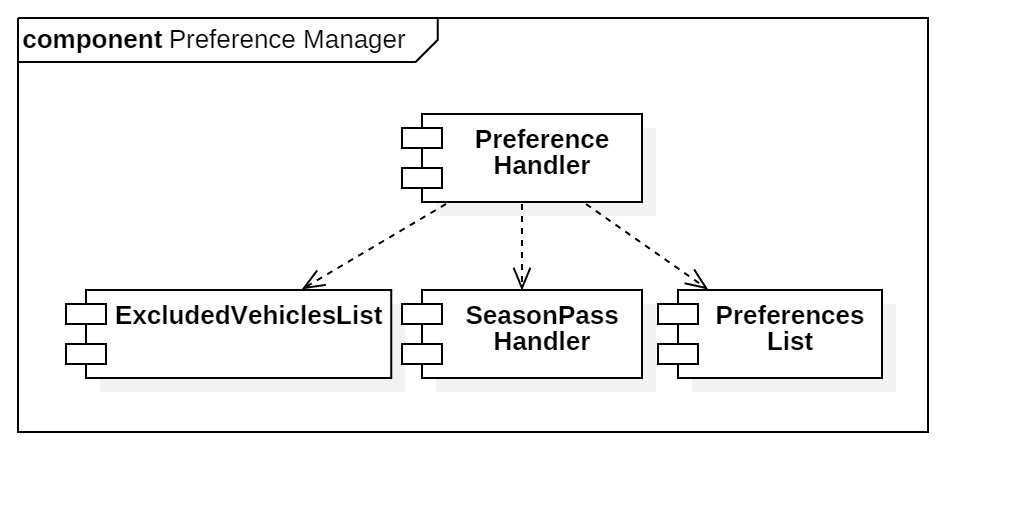
\includegraphics[scale = 0.2]{UML/componentDiagrams/preferenceManager}
	\end{figure}
	

\paragraph{Travlendar Server} 
	This component represents the \textit{Travlendar Server} whose purpose is to store User's preferences, access data and personal information. It is modeled by its 'DBMS' component, which stores Timetables and Preferences and the 'API Request Dispatcher', which forwards requests to external agents.

	\begin{figure}[H]
		\centering
		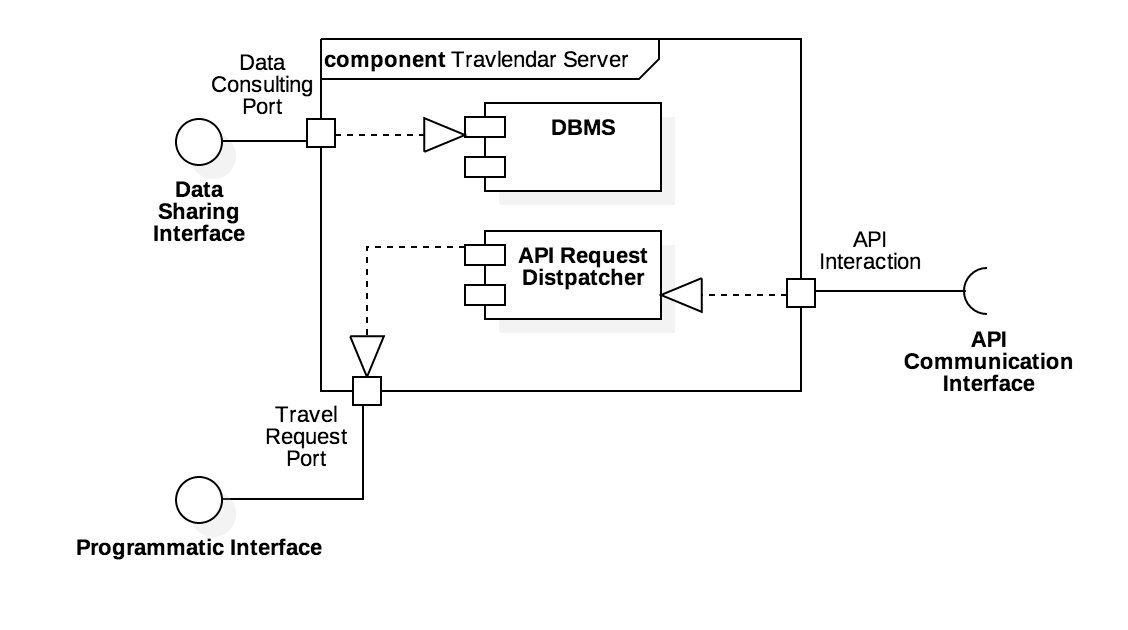
\includegraphics[scale = 0.2]{UML/componentDiagrams/travlendarServer}
	\end{figure}
	

\paragraph{Travel Logic Manager}
	This component is split into two sub-components: 'Scheduler' is the fundamental block that aims at scheduling and arranging User appointments and breaks via the the corresponding trips, 'DistanceManager' is the block whose purpose is to organize and present travel times to the scheduler in order to have them sorted out and well-managed.

	\begin{figure}[H]
		\centering
		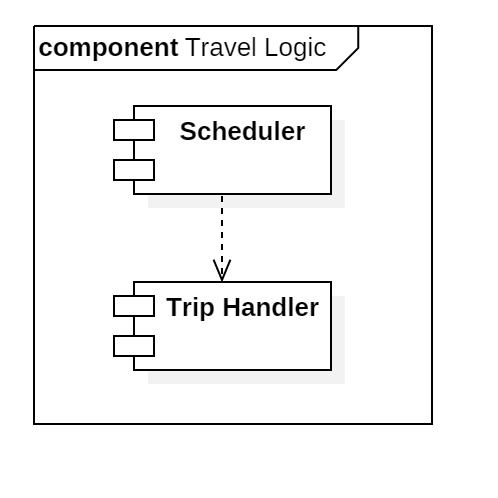
\includegraphics[scale = 0.2]{UML/componentDiagrams/travelLogic}
	\end{figure}
	

\paragraph{Payment Manager}
	This component deals with the recording of purchases and their associated credit cards.
	The sub-component 'Payment Handler' tracks purchase records and interacts with the required apps installed on the mobile device, while 'Purchase History' is an exploitable and rational organizations of the credit cards used by the user.

	\begin{figure}[H]
		\centering
		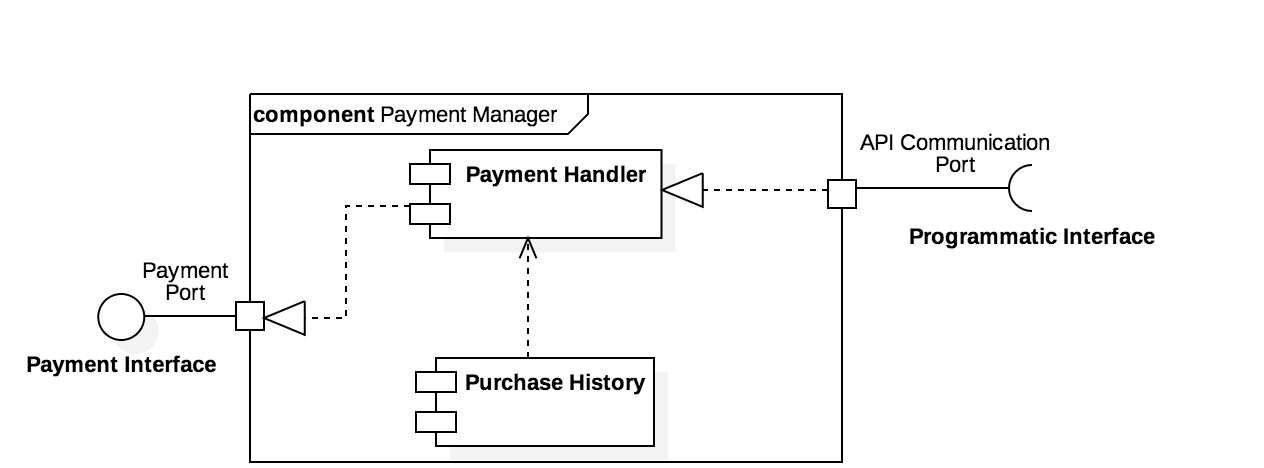
\includegraphics[scale = 0.2]{UML/componentDiagrams/paymentManager}
	\end{figure}
	

\paragraph{API Manager} 
	This component is critical in order to provide a functioning Travel Logic: it gathers the interactions with all external APIs.
	Here are listed the APIs the mobile application project starts with : Google Maps API, Google Transit API, Open Weather Map API, Car2Go and BikeMi API.
	The last couple is for reference only, as already pointed in the RASD. Naturally, the list of external services can be expanded.
	The 'Listener' component serves the purpose of forwarding requests and receives the desired inputs.
	
	\begin{figure}[H]
		\centering
		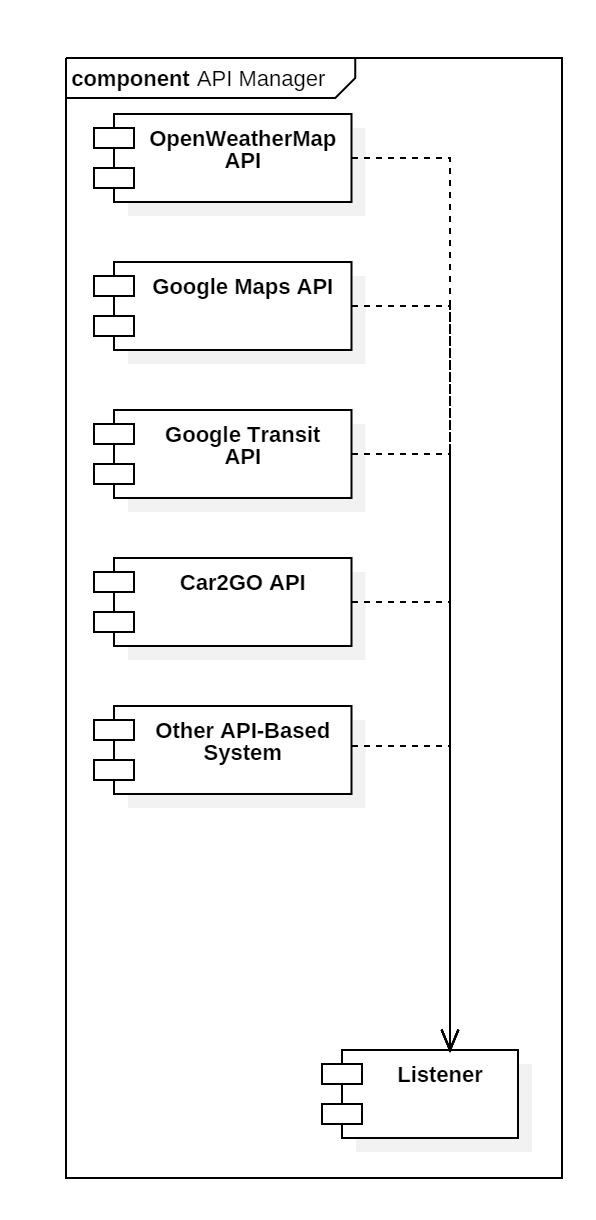
\includegraphics[scale = 0.2]{UML/componentDiagrams/APIManager}
	\end{figure}
	
	
\paragraph{Notification Manager}
	This component allows the notification system to warn users in the cases events partially or completely overlap according to the scheduler.

\paragraph{Localization Manager}
	This component represents the localization functionalities of the mobile application.
	
\begin{landscape}
	\begin{figure}
		\centering
		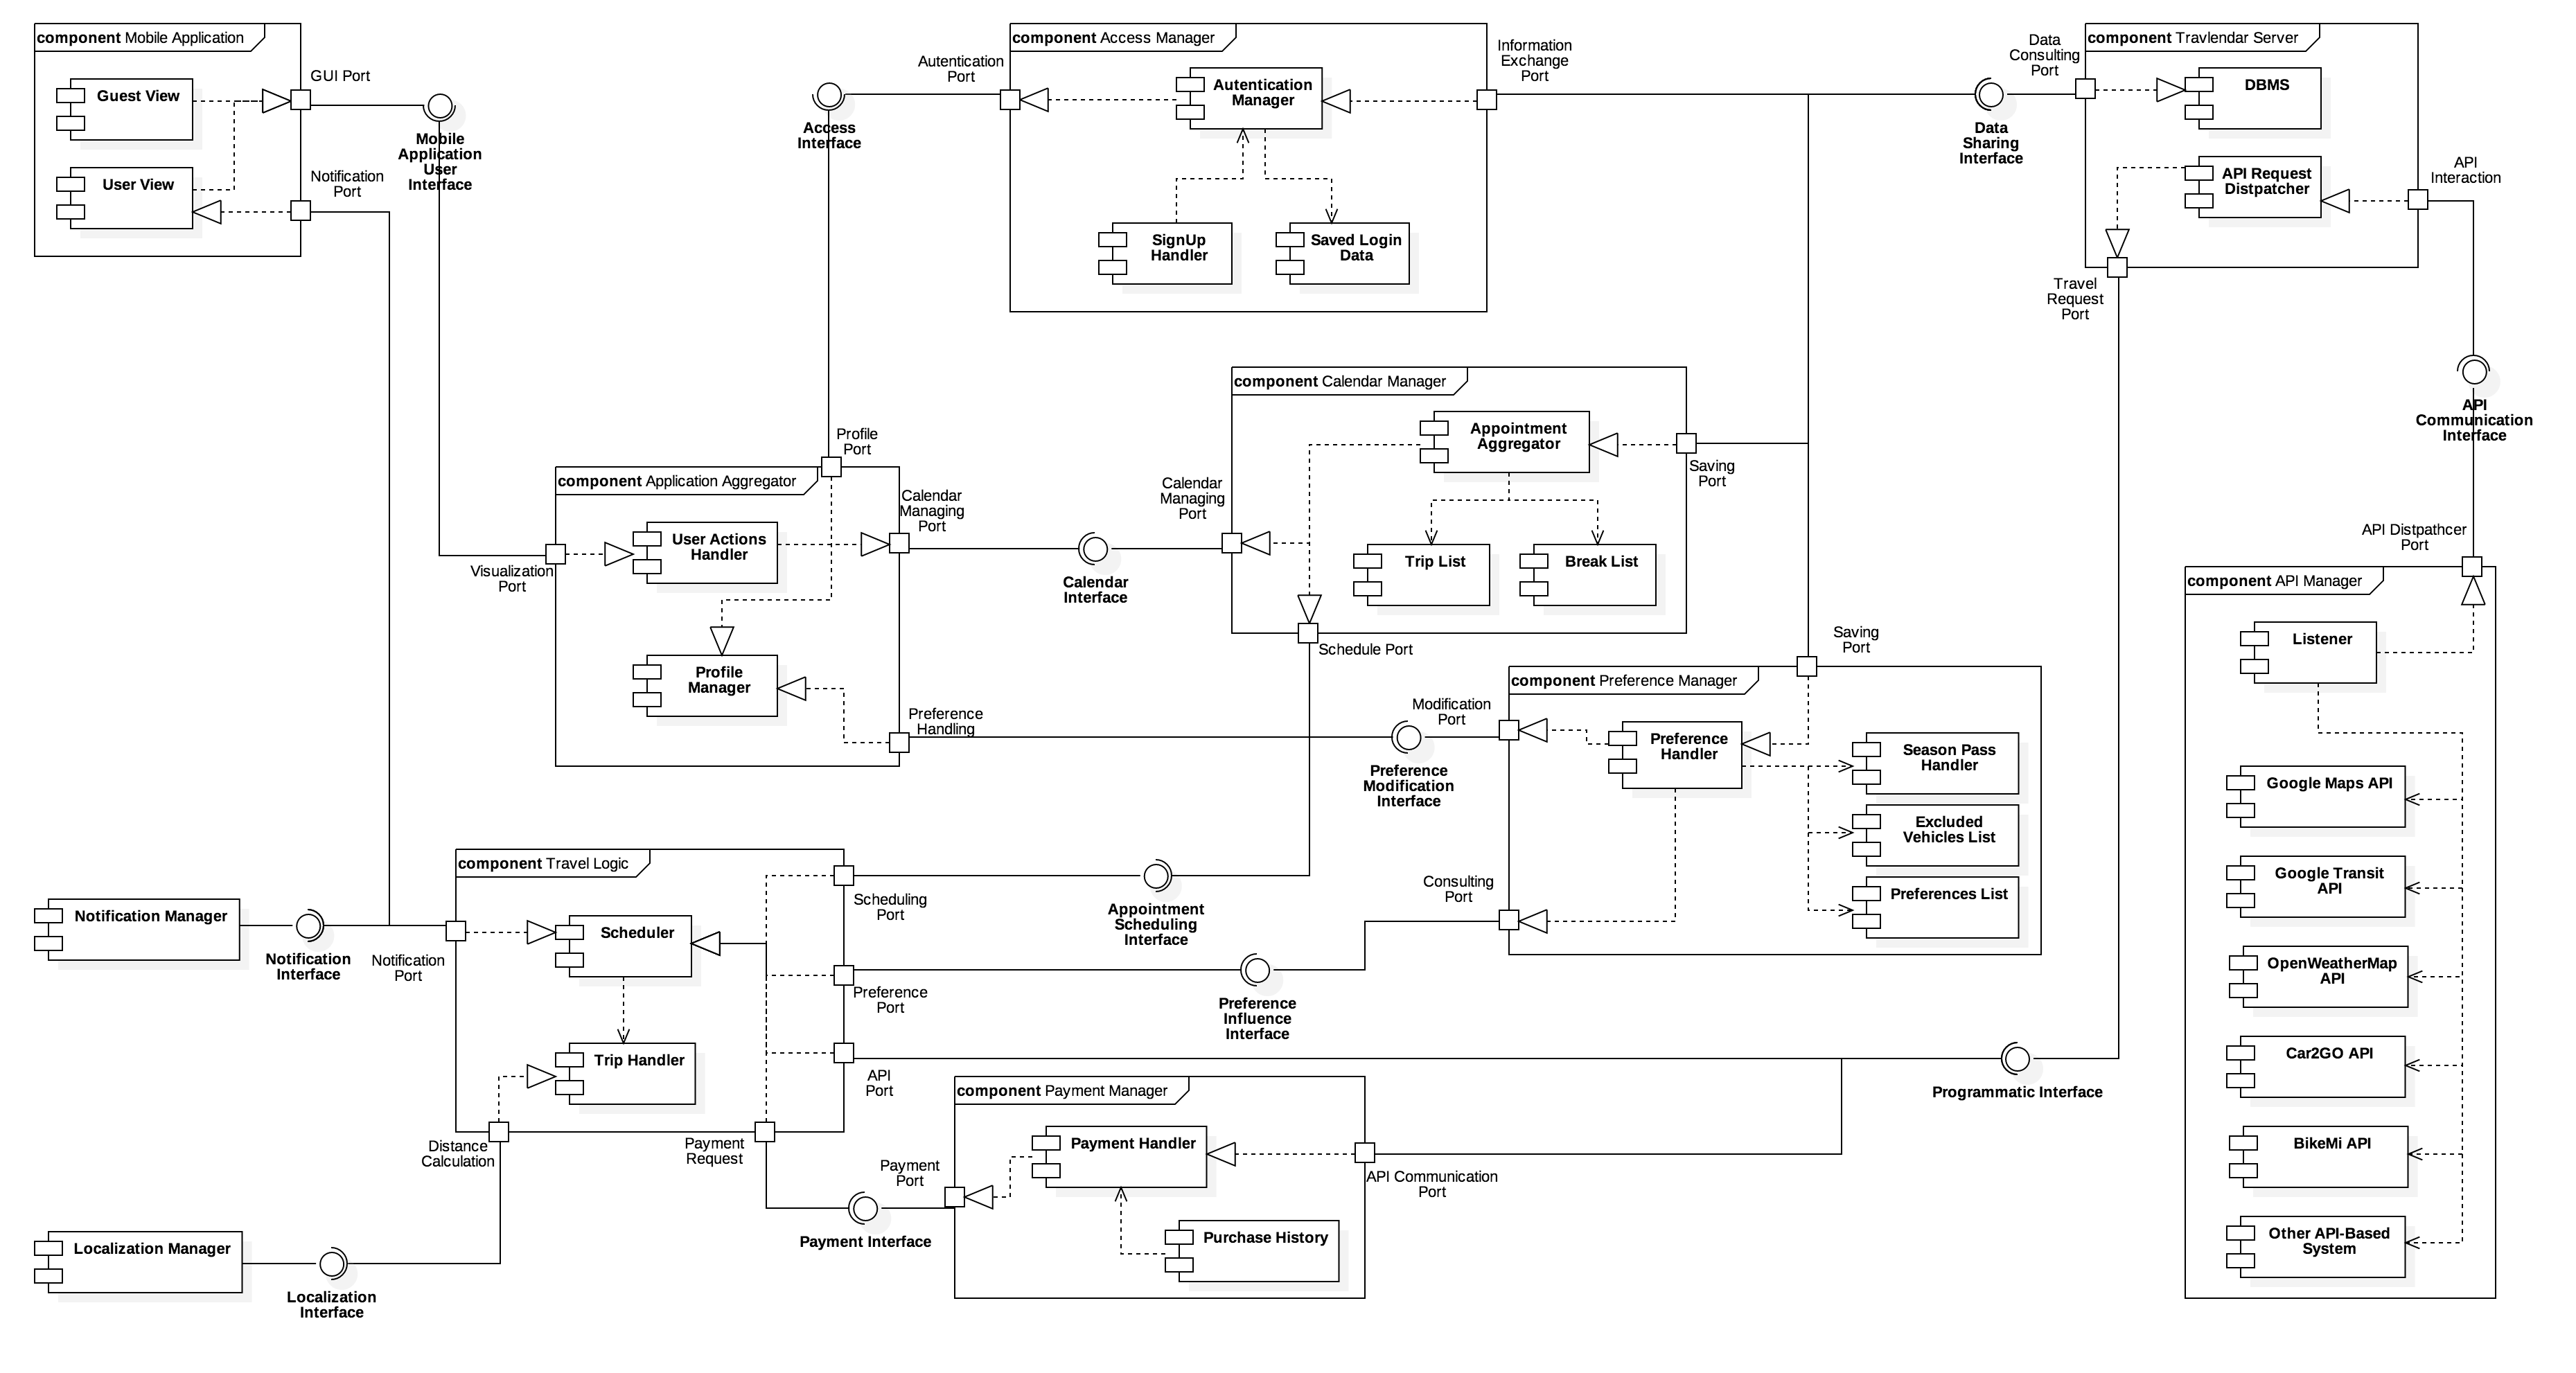
\includegraphics[height= 0.9\textheight]{UML/componentDiagrams/detailedLevel}
		\caption{Detailed level view}
		\label{detailedHighLevel}
	\end{figure}
\end{landscape}





	
\subsection{Deployment View}
	%The Component Diagram shown below describes the logical components of the system we are to develop, from a very high-level description on to a more detailed one. This diagram does not take into account the deployment phase, hence it doesn’t describe the logical layer of the system in terms of the physical tiers where it is deployed.

\begin{figure}[H]
		\centering
		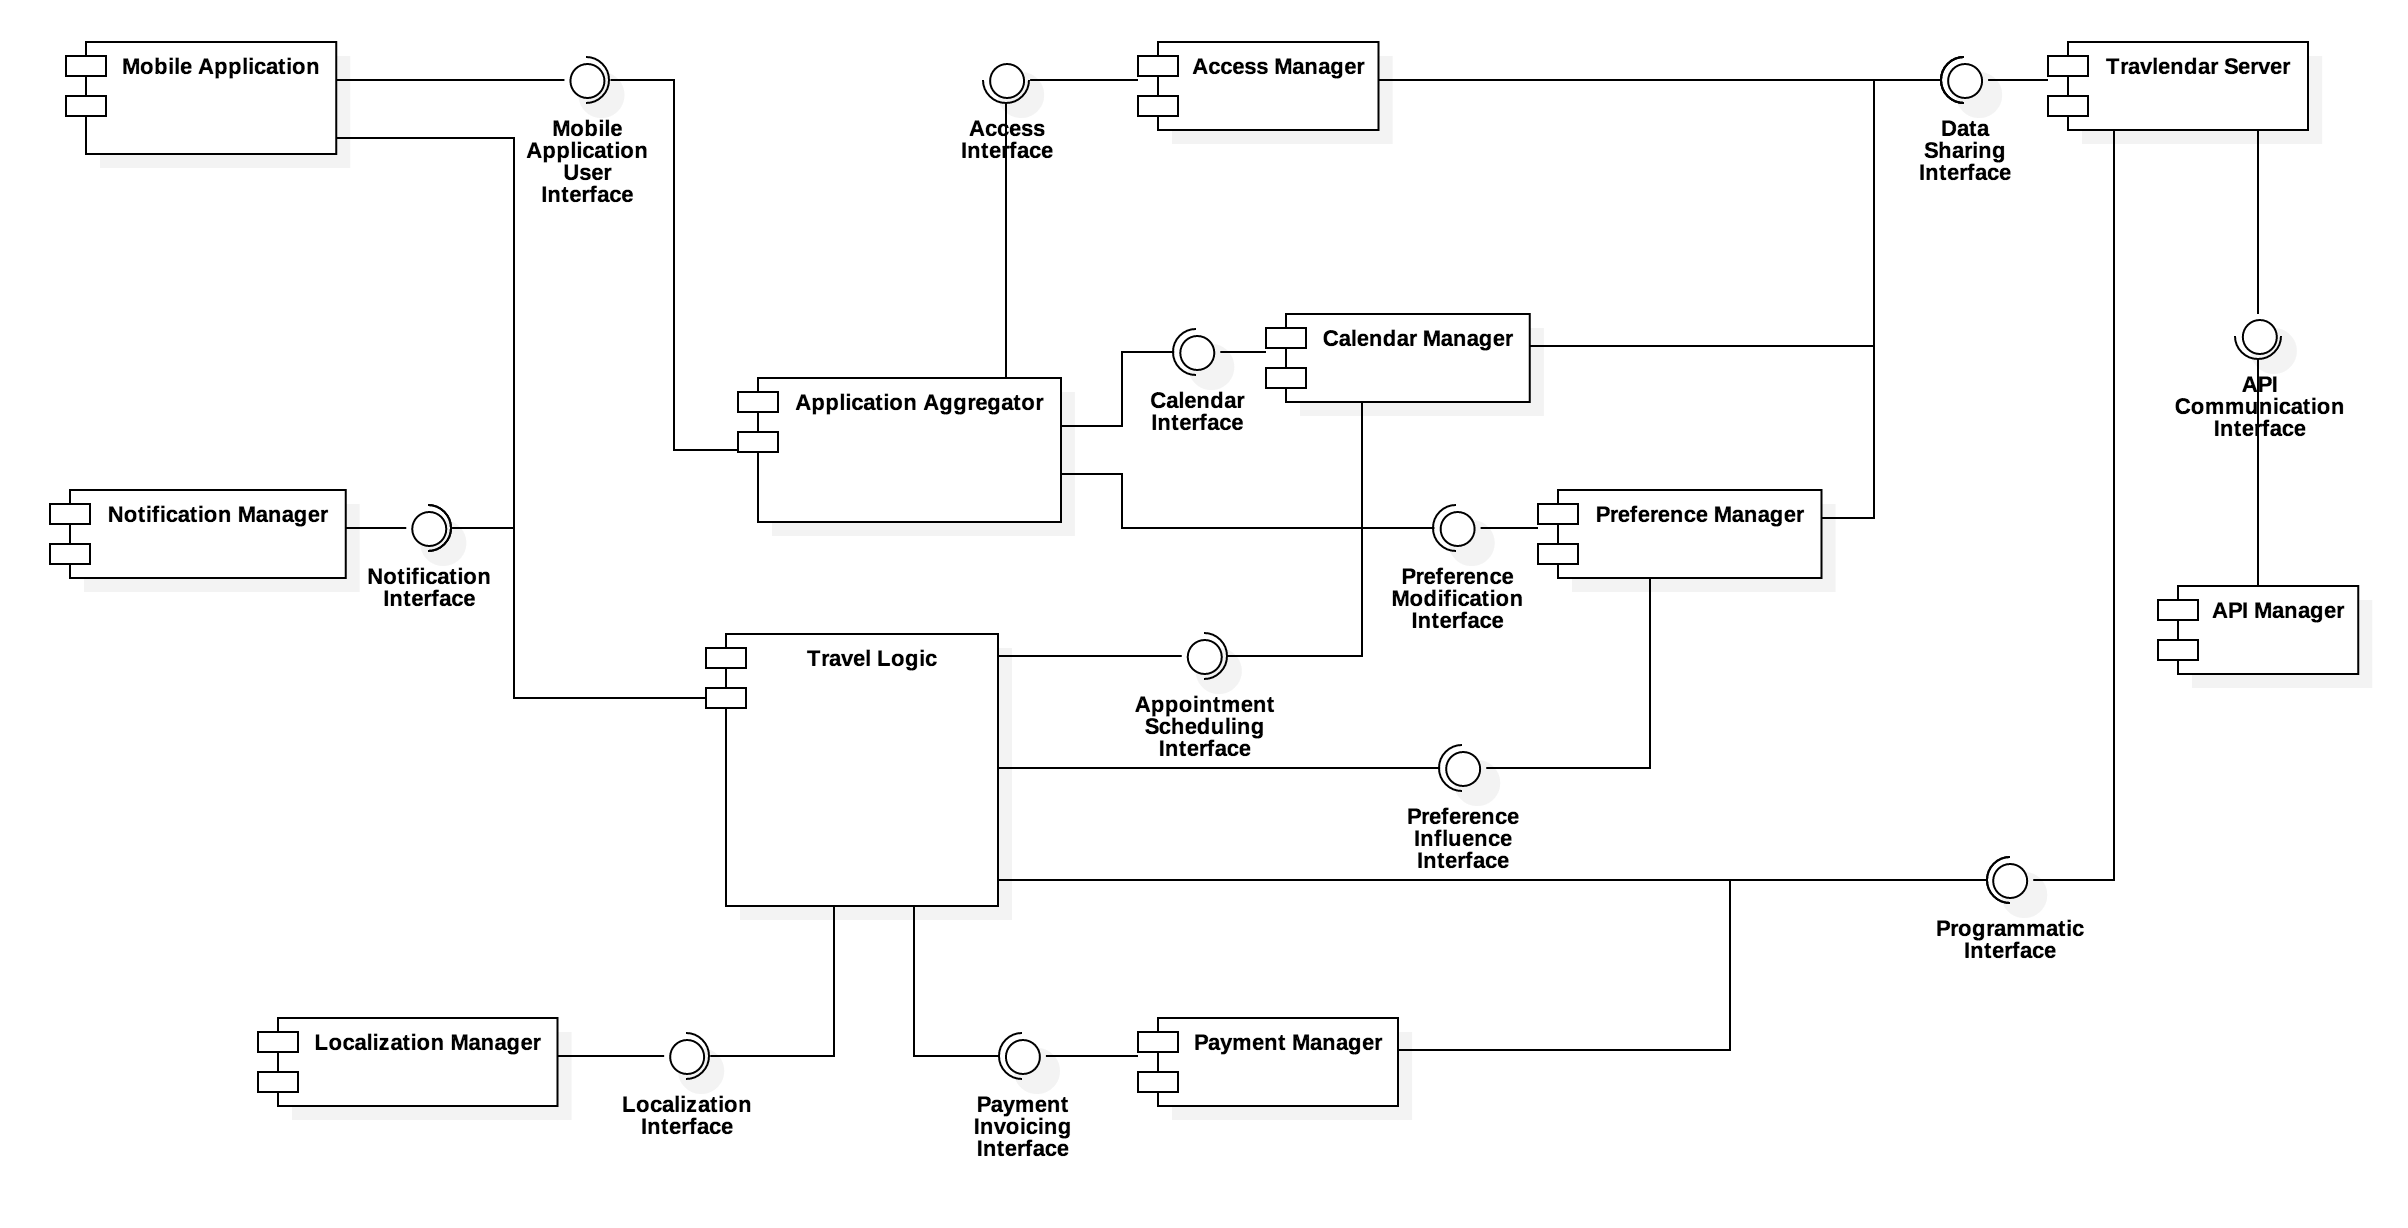
\includegraphics[width = \textwidth]{UML/componentDiagrams/highLevel}
		\caption{High level view}
		\label{componentHighLevel}
	\end{figure}

\paragraph{Mobile Application}
	This component represents the view of the User over its system. It’s split in two sub-components, Guest-view and User-view, which represents the two different ways an human interaction can be instaurated with the system.

	\begin{figure}[H]
		\centering
		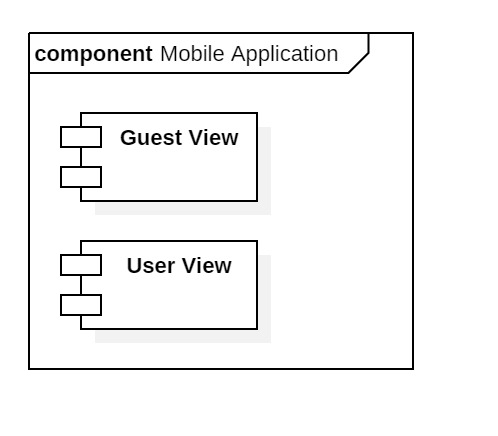
\includegraphics[scale = 0.2]{UML/componentDiagrams/mobileApplication}
	\end{figure}


\paragraph{Application Aggregator}
	This component works, unsuprisingly, as a collector of the different information \textit{Travlendar+} manages. It allows an easy management of every piece of information and allows us to avoid an high number of interfaces among the different components. 'Profile Manager' specifies the profile setting of the current user, while 'User Action Handler' allows us to register User's input.
	
	\begin{figure}[H]
		\centering
		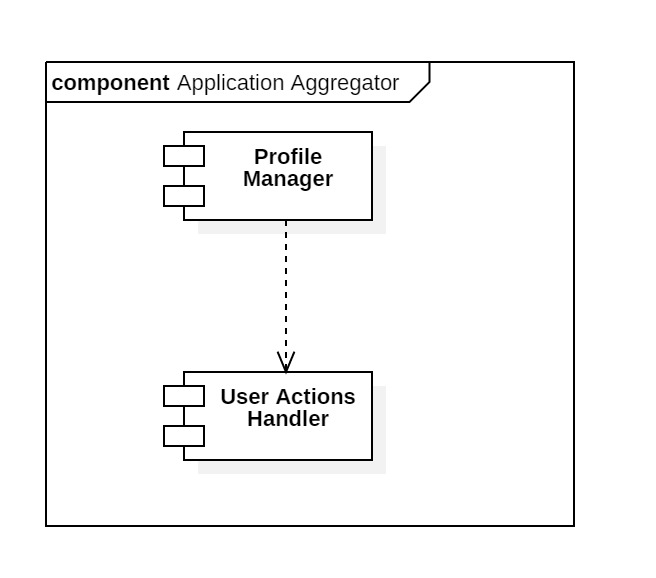
\includegraphics[scale = 0.2]{UML/componentDiagrams/applicationAggregator}
	\end{figure}
 
\paragraph{Calendar Manager}
	This component is divided into 'Appointments' and 'Breaks' sub-components, which track the appointments inserted by the User together with his breaks, and 'Trips', which is the list of trips arranged by the scheduler for every appointment. The sub-component 'Appointment Aggregator' serves the purpose of listing and presenting the content of the other two sub-components.
	
	\begin{figure}[H]
		\centering
		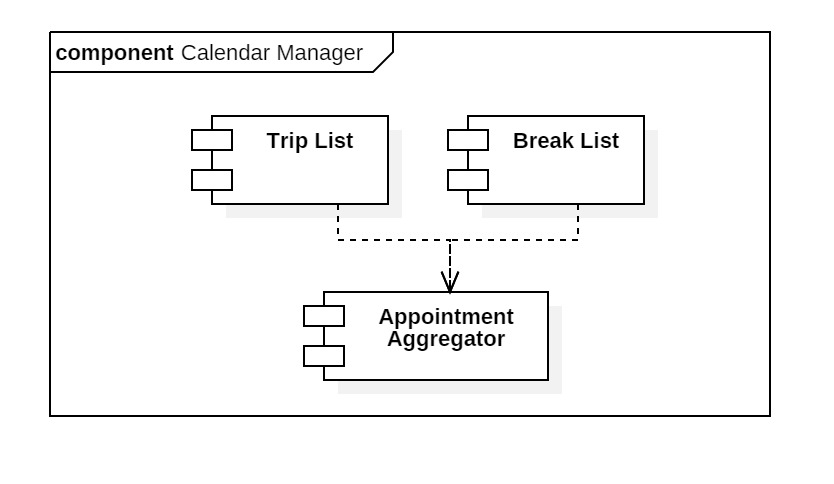
\includegraphics[scale = 0.2]{UML/componentDiagrams/calendarManager}
	\end{figure}
 

\paragraph{Preference Manager}
	This component serves the purpose of keeping track of the preferences expressed by the User. 'Season Pass Handler' takes care of storing season passes; 'Excluded Vehicles List' cuts off from the scheduler results involving a selection of banned transportation means, 'Preferences List' covers the remaining and wider spectrum of User's choices. 'Preference Handler' is the sub-component that manages the other ones and that communicates outside Preference Manager.

	\begin{figure}[H]
		\centering
		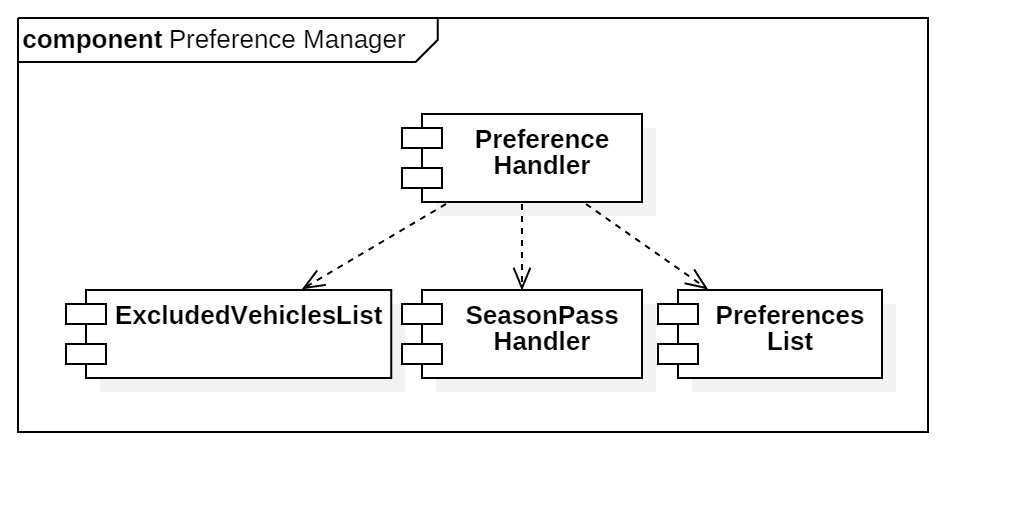
\includegraphics[scale = 0.2]{UML/componentDiagrams/preferenceManager}
	\end{figure}
	

\paragraph{Travlendar Server} 
	This component represents the \textit{Travlendar Server} whose purpose is to store User's preferences, access data and personal information. It is modeled by its 'DBMS' component, which stores Timetables and Preferences and the 'API Request Dispatcher', which forwards requests to external agents.

	\begin{figure}[H]
		\centering
		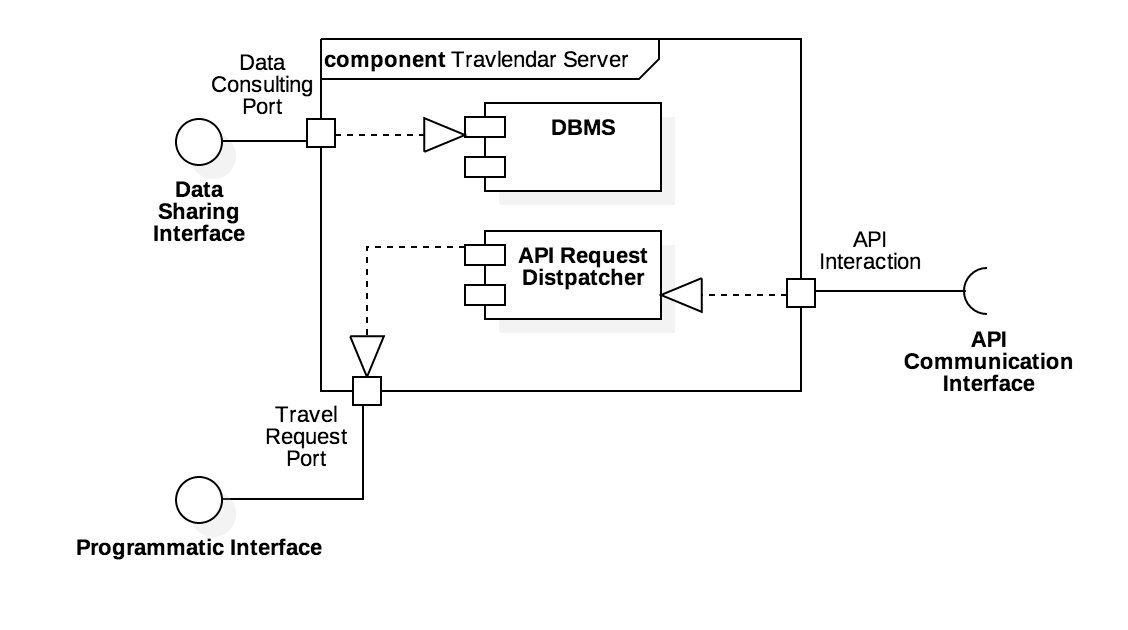
\includegraphics[scale = 0.2]{UML/componentDiagrams/travlendarServer}
	\end{figure}
	

\paragraph{Travel Logic Manager}
	This component is split into two sub-components: 'Scheduler' is the fundamental block that aims at scheduling and arranging User appointments and breaks via the the corresponding trips, 'DistanceManager' is the block whose purpose is to organize and present travel times to the scheduler in order to have them sorted out and well-managed.

	\begin{figure}[H]
		\centering
		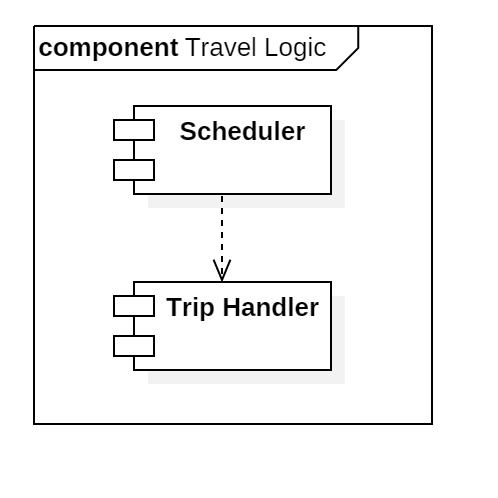
\includegraphics[scale = 0.2]{UML/componentDiagrams/travelLogic}
	\end{figure}
	

\paragraph{Payment Manager}
	This component deals with the recording of purchases and their associated credit cards.
	The sub-component 'Payment Handler' tracks purchase records and interacts with the required apps installed on the mobile device, while 'Purchase History' is an exploitable and rational organizations of the credit cards used by the user.

	\begin{figure}[H]
		\centering
		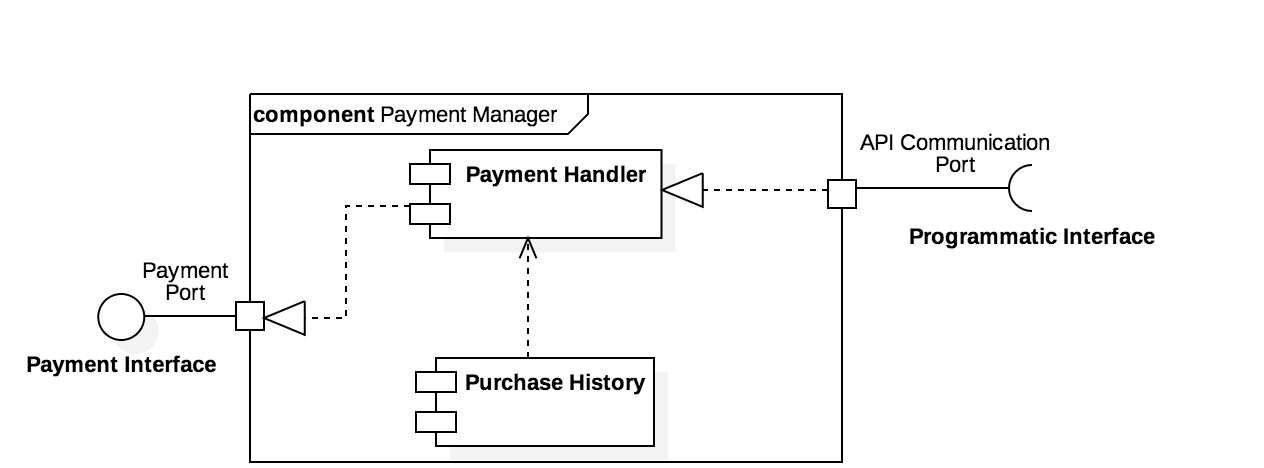
\includegraphics[scale = 0.2]{UML/componentDiagrams/paymentManager}
	\end{figure}
	

\paragraph{API Manager} 
	This component is critical in order to provide a functioning Travel Logic: it gathers the interactions with all external APIs.
	Here are listed the APIs the mobile application project starts with : Google Maps API, Google Transit API, Open Weather Map API, Car2Go and BikeMi API.
	The last couple is for reference only, as already pointed in the RASD. Naturally, the list of external services can be expanded.
	The 'Listener' component serves the purpose of forwarding requests and receives the desired inputs.
	
	\begin{figure}[H]
		\centering
		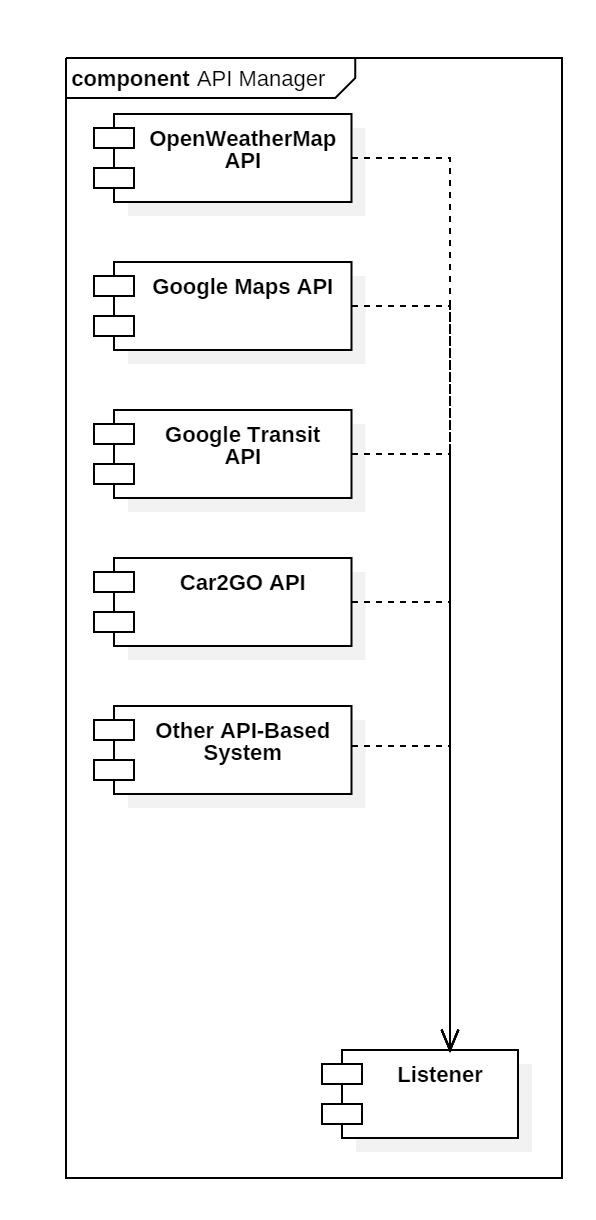
\includegraphics[scale = 0.2]{UML/componentDiagrams/APIManager}
	\end{figure}
	
	
\paragraph{Notification Manager}
	This component allows the notification system to warn users in the cases events partially or completely overlap according to the scheduler.

\paragraph{Localization Manager}
	This component represents the localization functionalities of the mobile application.
	
\begin{landscape}
	\begin{figure}
		\centering
		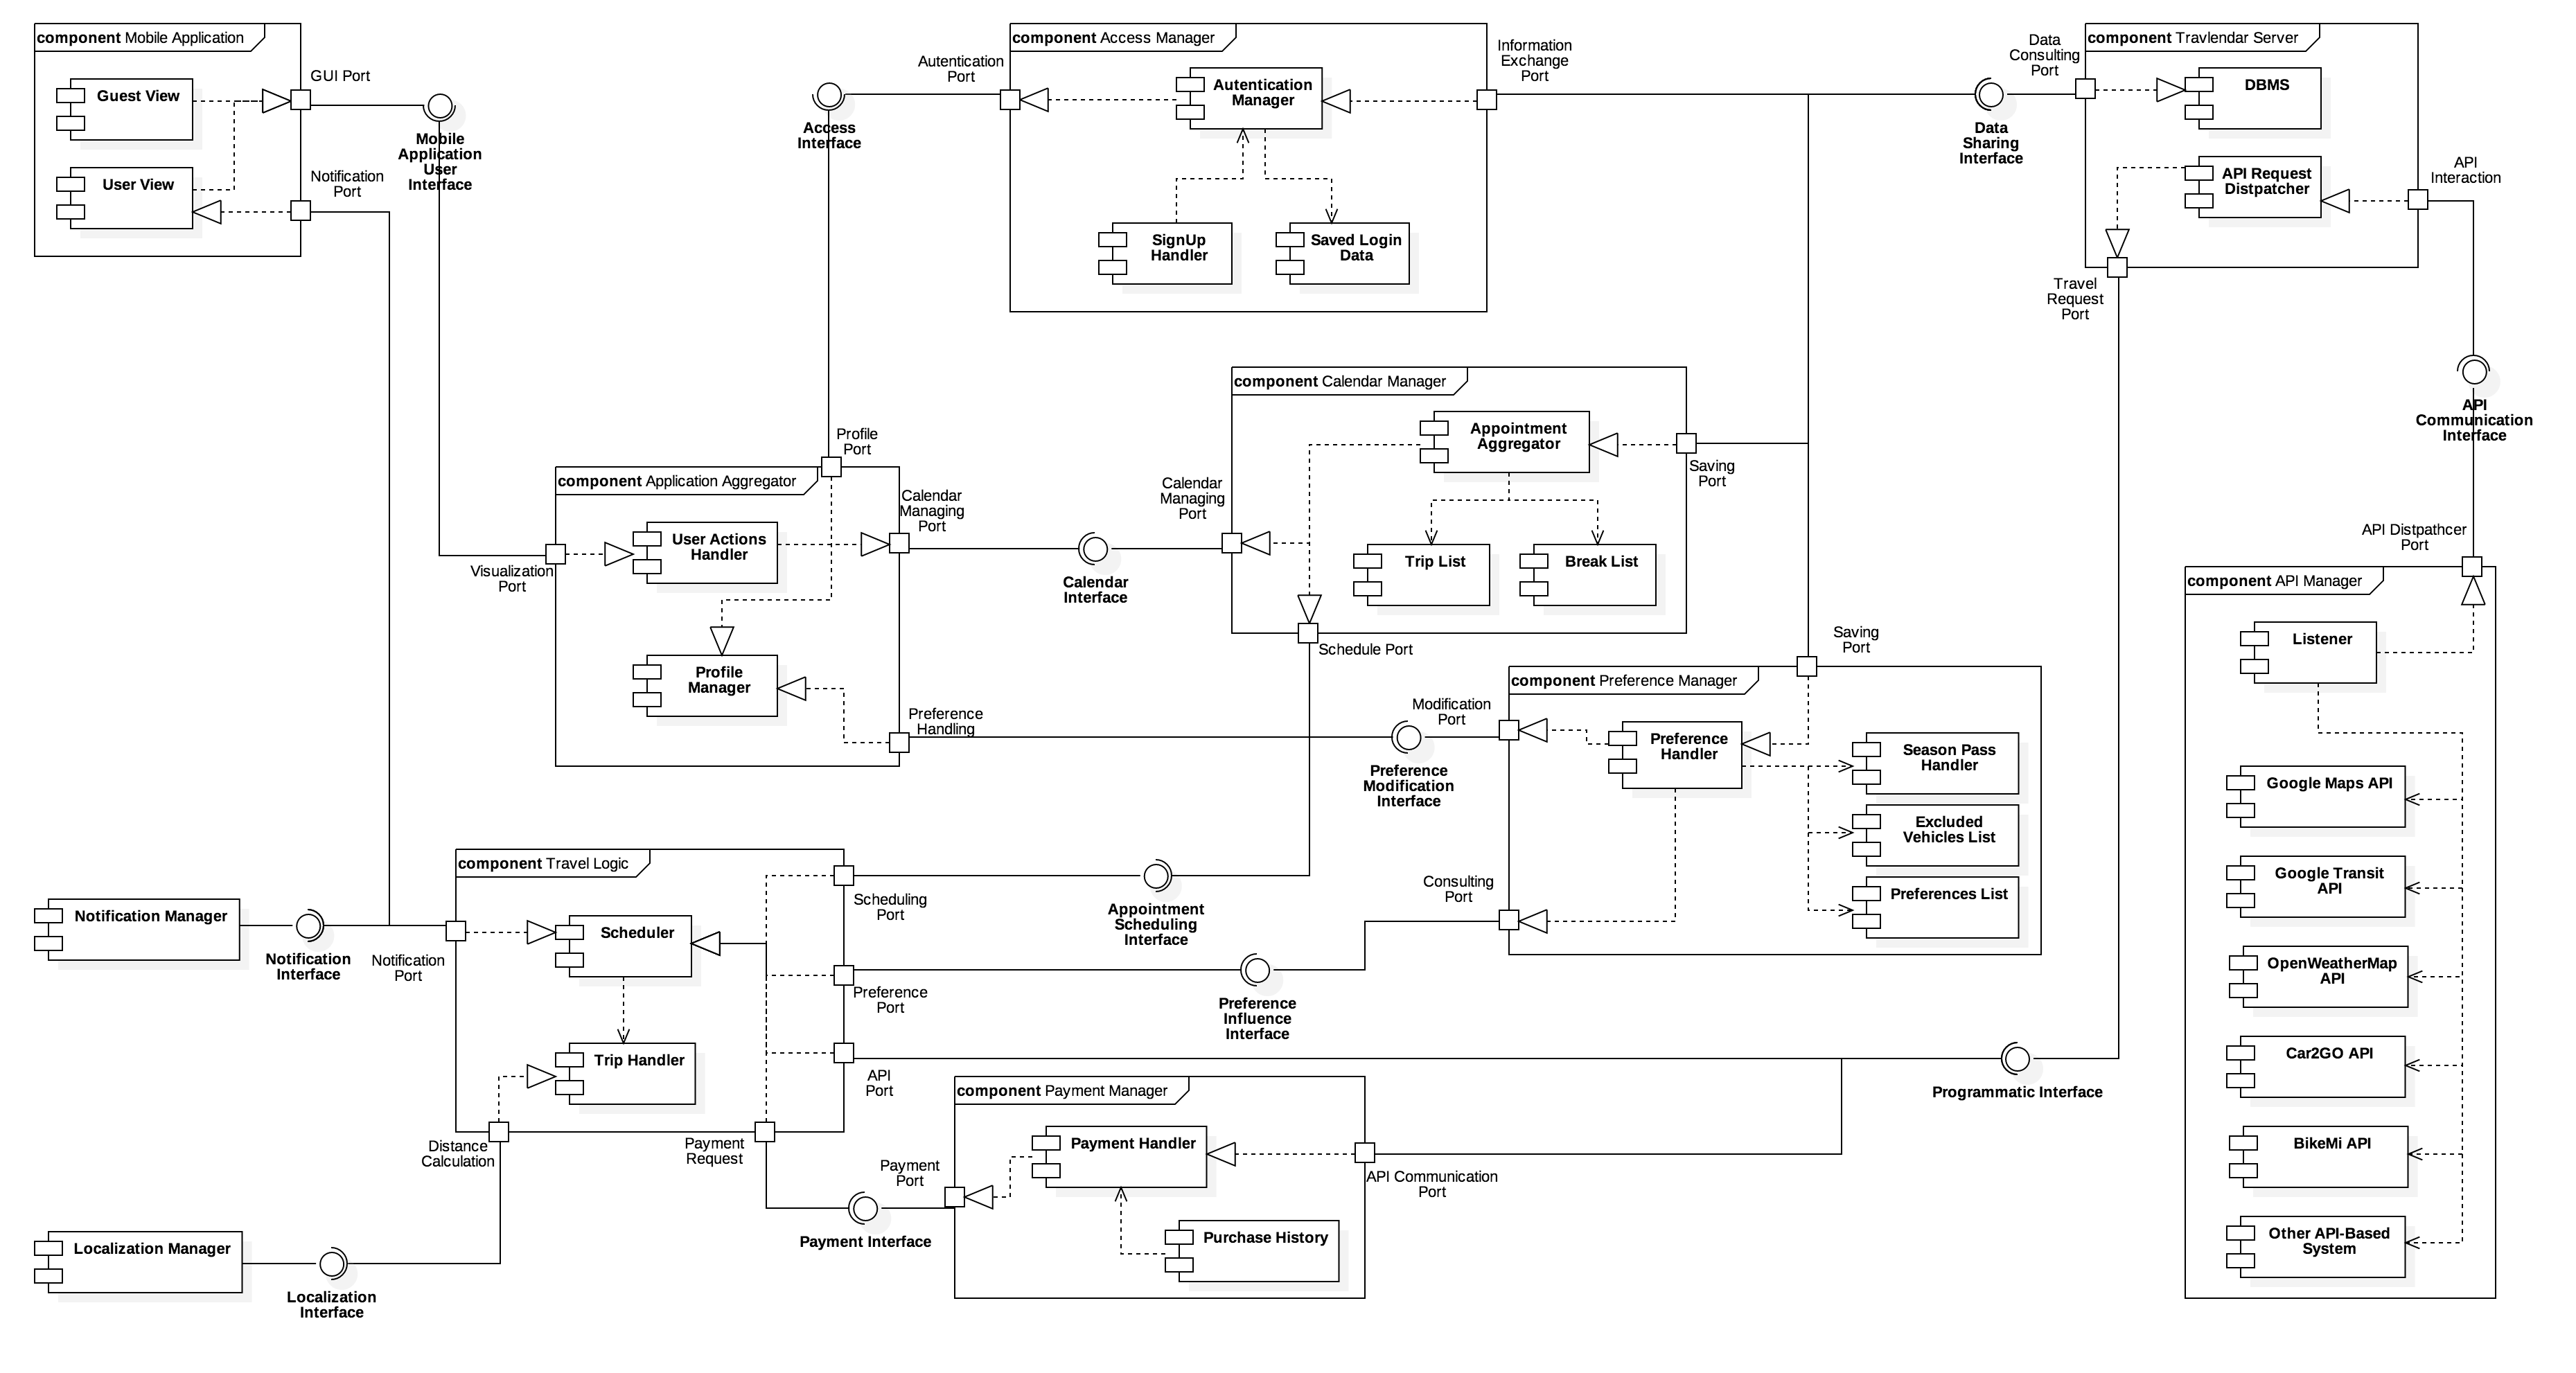
\includegraphics[height= 0.9\textheight]{UML/componentDiagrams/detailedLevel}
		\caption{Detailed level view}
		\label{detailedHighLevel}
	\end{figure}
\end{landscape}





	
\subsection{Runtime view}
	%\input{subsections/section2/rutimeView.tex}

\subsection{Component Interfaces}
	%In this section we will show the component Interfaces. For each one are reported the main functionalities.
Nevertheless we need to keep in mind that in further implementations these functions can be splitted into less complex ones.

\begin{figure}[H]

	\begin{subfigure}[t]{0.3\linewidth}
		\centering
		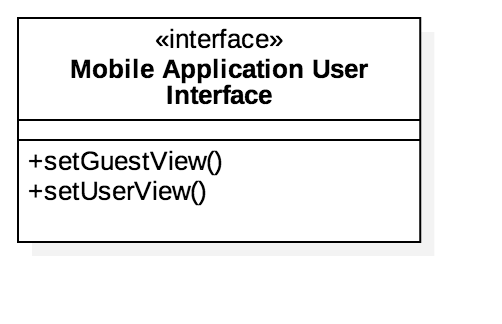
\includegraphics[width=\linewidth]{UML/Interfaces/mobileApplicationUserInterface}
		\caption{Mobile Application User Interface}
	\end{subfigure}
	~
	\begin{subfigure}[t]{0.3\linewidth}
		\centering
		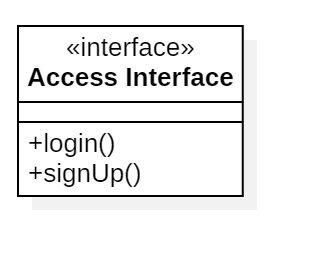
\includegraphics[width=\linewidth]{UML/Interfaces/accessInterface}
		\caption{Access Interface}
	\end{subfigure}
	~	
	\begin{subfigure}[t]{0.3\linewidth}
		\centering
		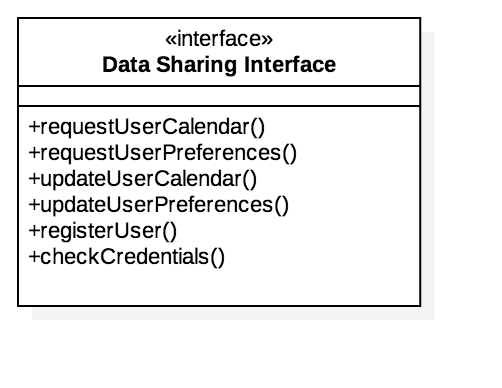
\includegraphics[width=\linewidth]{UML/Interfaces/dataSharingInterface}
		\caption{Daba Sharing Interface}
	\end{subfigure}
	\hfill
	\vskip0.75cm
	
	
	\begin{subfigure}[t]{0.3\linewidth}
		\centering
		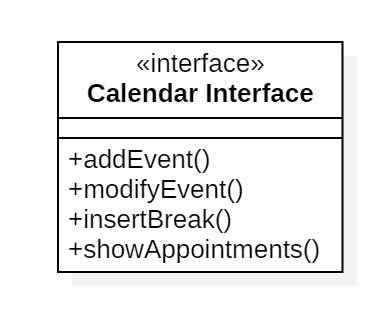
\includegraphics[width=\linewidth]{UML/Interfaces/calendarInterface}
		\caption{Calendar Interface}
	\end{subfigure}
	~
	\begin{subfigure}[t]{0.3\linewidth}
		\centering
		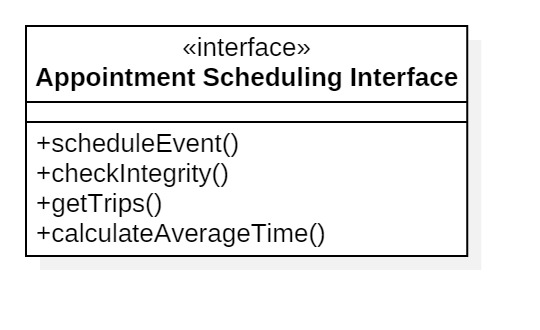
\includegraphics[width=\linewidth]{UML/Interfaces/appointmentSchedulingInterface}
		\caption{Appointment Scheduling Interface}
	\end{subfigure}
	~
	\begin{subfigure}[t]{0.3\linewidth}
		\centering
		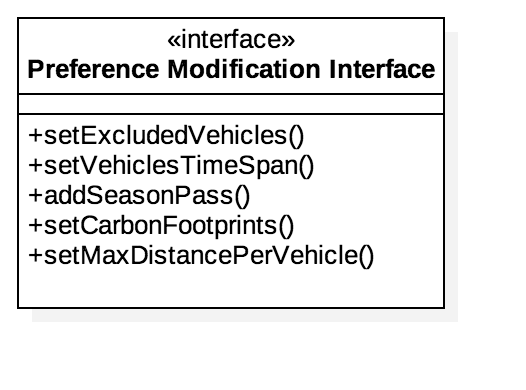
\includegraphics[width=\linewidth]{UML/Interfaces/preferenceModificationInterface}
	\caption{Preference Modification Interface}
	\end{subfigure}
	\hfill
	\vskip0.75cm
	
	
	\begin{subfigure}[t]{0.3\linewidth}
		\centering
		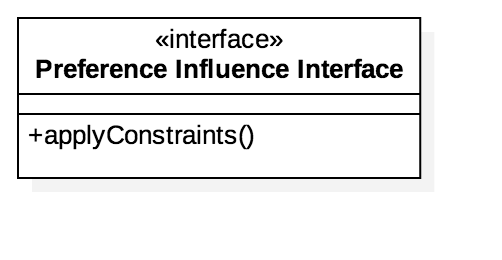
\includegraphics[width=\linewidth]{UML/Interfaces/preferenceInfluenceInterface}
		\caption{Preference Influence Interface}
	\end{subfigure}
	~
	\begin{subfigure}[t]{0.3\linewidth}
		\centering
		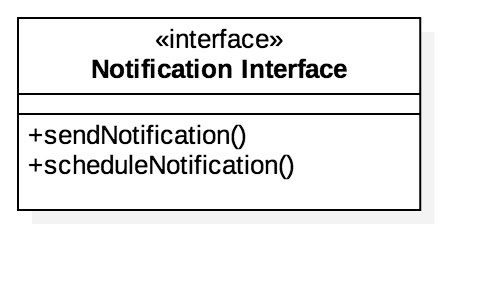
\includegraphics[width=\linewidth]{UML/Interfaces/notificationInterface}
		\caption{Notification Interface}
	\end{subfigure}
	~
	\begin{subfigure}[t]{0.3\linewidth}
		\centering
		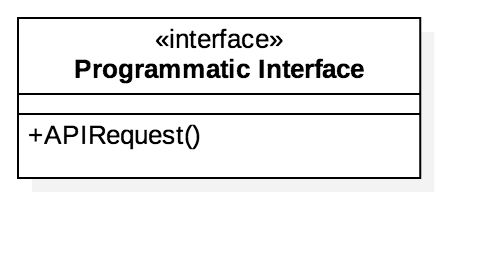
\includegraphics[width=\linewidth]{UML/Interfaces/programmaticInterface}
		\caption{Programmatic Interface}
	\end{subfigure}
\end{figure}	


\begin{figure}[H]\ContinuedFloat
	\begin{subfigure}[t]{0.3\linewidth}
		\centering
		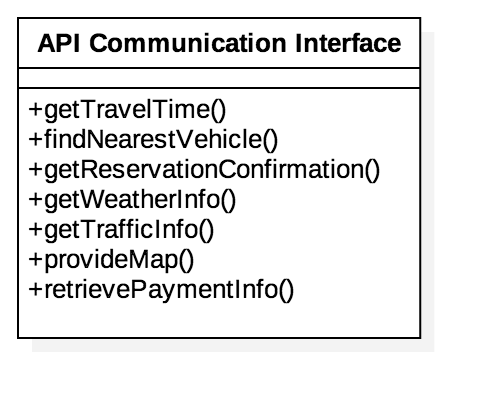
\includegraphics[width=\linewidth]{UML/Interfaces/APICommunicationInterface}
		\caption{API Communication Interface}
	\end{subfigure}
	~
	\begin{subfigure}[t]{0.3\linewidth}
		\centering
		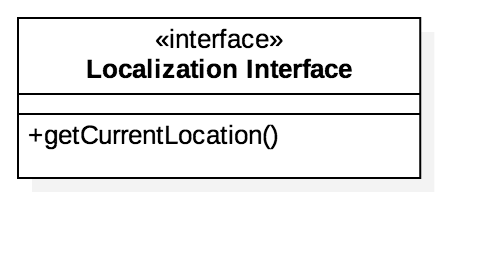
\includegraphics[width=\linewidth]{UML/Interfaces/localizationInterface}
		\caption{Localization Interface}
	\end{subfigure}
	~
	\begin{subfigure}[t]{0.3\linewidth}
		\centering
		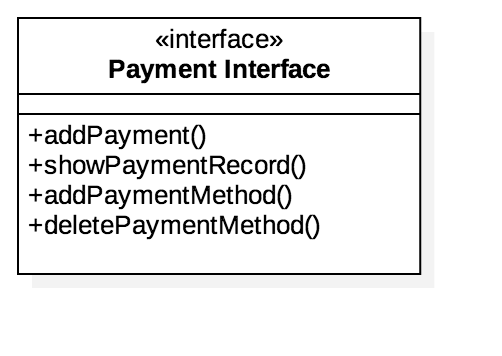
\includegraphics[width=\linewidth]{UML/Interfaces/paymentInterface}
		\caption{Payment Interface}
	\end{subfigure}
	
	\caption{List of Interfaces}
\end{figure}

\subsection{Architectural Styles}
	
[Architectural Style]

For our system architecture we adopt a 3-tier client/server architecture : we'll have a Mobile Application Clients, a Travlendar
 Server and a Data Storage Layer.


Mobile Application Clients : This layer is represented by the Travlendar+ Application, a thick client and an interactive and dinamic GUI.
The application will be written in Java for increased portability and will be able both to geo-localize its user and to communciate with the core of the travel : this is the foundation of information synching and requests forwarding to APIs.

Travlendar+ Server : The business Server runs the business logic. Its main duty is to forward requests of the users to the Data layer and external APIs while saving all necessary users' preferences and timetables. These operations are executed under a microservice architectural pattern.

The Data Layer : This layer comprehends both the DBMS which stores and manages users' preferences and timetables and the external service agents (objects which call external services). In the former case it is required the capability of providing data through SQL queries using ODBC protocol, while in the latter it is required a good implementation of the ad-hoc functions of the external APIs.
(link Microsoft)

Patterns

Pattern are mostly required to smooth the construction of our system. In particular, we'll be using a MVC (Model - View - Control) Pattern for our mobile application, Adapter (??), Client/Server and Single Instance component.

MVC is used to define our Java mobile application : the view will be the dynamic GUI, the Travel Logic the control and the model will be the data received from the APIs and the locally stored timetables and trips.


Single Instance component will be mostly useful when treating the components of the mobile application : components like Access Manager or Travel Logic will be the ones mainly touched by this pattern.

Client/Server pattern is the one we adopted to shape the interactions between our mobile application (the client) and the Travlendar+ Server (i.e, the server). Reasons for adoption have mainly been the simplicity and widespread use of the model.


%Vecchia parte di Michele!
In particolare ci serviremo del pattern MVC (Model View Control) molto utile perchè ci permette di separare la logica Business dalla logica di Presentazione. In questo caso il Database interpreterà il ruolo del Model, Mobile Application interpreterà il ruolo di View, e il Server sarà il Control. 
